% We begin by calling the workreport class which includes all the
% definitions for the macros we will use.
\documentclass[ece]{uw-wkrpt}

% We will use some packages to add functionality
\usepackage{graphicx} % Include graphic importing

% Now we will begin writing the document.
\begin{document}

%%%%%%%%%%%%%%%%%%%%%%%%%%%%%%%%%%%%%%%%%%%%%%%%%%%%%%%%%%%%%%%%%%%%%
%% IMPORTANT INFORMATION
%%%%%%%%%%%%%%%%%%%%%%%%%%%%%%%%%%%%%%%%%%%%%%%%%%%%%%%%%%%%%%%%%%%%%

%% First we, should create a title page.  This is done below:
% Fill in the title of your report.
\title{Design of an Automotive Center Stack for the EcoCAR 2 Advanced Vehicle
Technology Competition}

% Fill in your name.
\author{Eric Evenchick}

% Fill in your student ID number.
\uwid{20339729}

% Fill in your home address.
\address{184 Kehoe St,\\*
         Ottawa, ON\ \ K2B 6A5}

% Fill in your employer's name.
\employer{University of Waterloo Alternative Fuels Team}

% Fill in your employer's city and province.
\employeraddress{Waterloo, ON}

% Fill in your school's name.
\school{University of Waterloo}

% Fill in your faculty name.
\faculty{Faculty of Engineering}

% Fill in your e-mail address.
\email{eric@evenchick.com}

% Fill in your term.
\term{3B}

% Fill in your program.
\program{Electrical Engineering}

% Fill in the department chair's name.
\chair{Manoj Sachdev}

% Fill in the department chair's mailing address.
\chairaddress{E\&CE Department,\\*
              University of Waterloo,\\*
	      Waterloo, ON\ \ N2L 3G1}

\selfstudy{Self Study}

% If you are writing a "Confidential 1" report, uncomment the next line.
%\confidential{Confidential-1}

% If you want to specify the date, fill it in here.  If you comment out
% this line, today's date will be substituted.
%\date{April 26, 2003}

% Now, we ask LaTeX to generate the title.
\maketitle

%%%%%%%%%%%%%%%%%%%%%%%%%%%%%%%%%%%%%%%%%%%%%%%%%%%%%%%%%%%%%%%%%%%%%
%% FRONT MATTER
%%%%%%%%%%%%%%%%%%%%%%%%%%%%%%%%%%%%%%%%%%%%%%%%%%%%%%%%%%%%%%%%%%%%%
%% \frontmatter will make the \section commands ignore their numbering,
%% it will also use roman page numbers.
\frontmatter

% After this, we must create a letter of submission.
\begin{letter}
This report, entitled ``\thetitle", was prepared during my \theterm{} work term
for my WKRPT 300 course. This is a self study report, and covers work that I
performed with the University of Waterloo Alternative Fuels Team.

The report covers my work as part of the center stack development group of the
Alternative Fuels Team, which is responsible for designing a human-machine
interface for the team's hybrid vehicle. This report covers the design and
development of the system. It has been written for the team, as well as
to satisfy my Work Term report requirements.

I have had no direct assistance from anyone with the preparation of this report. 
However I have made use of Freescale's application notes to implement the
design, and the GUI which is covered in this report was primarily
implemented by Rickey Si Rui Wang.

% Note that I do not need to type out the boilerplate confirmation,
% nor do I need to write a signature block.  This is generated for me.
% We are now finished with the letter.
\end{letter}

% We continue with required sections, such as the Contributions and Summary
\begin{onehalfspacing}
\section{Contributions}

The University of Waterloo Alternative Fuels Team is a Waterloo student
team that participates in Advanced Vehicle Technology Competitions. Currently,
the team is taking part in the EcoCAR 2 competition.

For this project, I worked with a small group of students, with the main goal of 
implementing a center stack for the vehicle. This piece of hardware consists of a
touchscreen and an embedded computer that allows the driver to interact with the
vehicle.

My tasks were to lead the project, get the low level software working on the
hardware, and write an abstraction level to allow developers to access the car's
internal network.

I would like to thank several members of the University of Waterloo Alternative
Fuels Team for their contributions.
Rickey Si Rui Wang, who developed the graphical user interface for the system,
Gurhari Singh, who leads the University of Waterloo Alternative Fuels Team, and
finally Dr. Roydon Fraser, who is the team's faculty advisor.

This report is related to the work since it details the design that was used for
the center stack software. It shows the use of engineering skills to design and
implement an embedded system for a real world application.

In the broader scheme of things, the resulting system lead to the creation of
tools that are useful for designing Linux based systems, and for interacting
with vehicles from a Linux based system. These tools will be explained in the
report, and will be released as open source projects for others looking to
implement similar solutions.

\section{Summary}

The purpose of this report is to outline the design of a center stack
for the University of Waterloo Alternative Fuels Team's EcoCAR 2 competition
vehicle. The center stack is a piece of hardware that lets the driver interact
with the vehicle. The scope of the report covers the hardware used to implement the
stack, and the software that has been written to achieve the desired
functionality.

The main points covered in this report are a summary of the hardware used, the
implementation of the operating system on the hardware, the software used
communicate with the car, and the graphical user interface for the system.

The major conclusions of this report is that the University of Waterloo
Alternative Fuels Team now has a base system to build their center stack around.
The implementation is modular, and will simplify future development by handling
the lower level requirements of the system. These conclusions are covered in
further detail in the conclusions section of this report.

The major recommendations of this report are that there are many improvements that
can be made to the system. This includes improvements to the hardware and
software used to build the system. These recommendations are covered in depth in
the recommendations section of this report.

\end{onehalfspacing}

% Next, we need to make a Table of Contents, List of Figures and 
% List of Tables.  You will most likely need to run LaTeX twice to
% get these correct.  The first pass for LaTeX to figure out the
% labels, and the second pass to put in the right references.
\tableofcontents
\listoffigures
\listoftables

%%%%%%%%%%%%%%%%%%%%%%%%%%%%%%%%%%%%%%%%%%%%%%%%%%%%%%%%%%%%%%%%%%%%%
%% REPORT BODY
%%%%%%%%%%%%%%%%%%%%%%%%%%%%%%%%%%%%%%%%%%%%%%%%%%%%%%%%%%%%%%%%%%%%%
%% \main will make the \section commands numbered again,
%% it will also use arabic page numbers.
\mainmatter

\section{Introduction}\label{sec:intro}

For the EcoCAR 2 Advanced Vehicle Technology Competition, the University of
Waterloo Alternative Fuels Team (UWAFT) was tasked with designing, implementing,
and testing a vehicle to reduce environmental impact while maintaining or
improving consumer acceptability. The competition spans three years. In the
first year, the team performs design and modeling tasks to design and justify
the vehicle architecture that they have chosen to implement. In year two, the
team builds a prototype vehicle. In the third year, the team attempts to get the 
vehicle to a consumer ready state, ensuring that the vehicle is acceptable for
consumers looking to purchase a modern automobile. UWAFT is designing an
ethanol-electric series hybrid vehicle for the competition, which is currently
in its second year.

One component of the vehicle design is a center stack: a device that allows the
driver to see critical information and interact with the vehicle. This center
stack is required to display certain signals from the vehicle's Controller Area
Network (CAN) bus in order to ensure that the vehicle is in a safe state. Since
the vehicle is in a prototype state, it is critical to monitor various signals
to ensure that it is operating correctly. These signals include:

\begin{itemize}
    \item battery state of charge,
    \item battery current,
    \item battery temperature,
    \item high voltage isolation resistance,
    \item engine status,
    \item engine temperature,
    \item motor torque.
\end{itemize}

The center stack also has the potential to increase the consumer acceptability
of the vehicle by providing new features. These features could include
navigation, entertainment, and telematics.

This report will detail the design of the center stack system. It will first
explain the hardware used to implement the system. Next, the operating system
used to build the system will be discussed. The low level communications
software design will be then discussed. The graphical user interface (GUI) will
be explained. Finally, conclusions and recommendations for the project will be
provided.

\section{Hardware}

The project was sponsored by Freescale Semiconductor, who provided hardware and
technical support. A Smart Application Blueprint for Rapid Engineering (SABRE)
platform based on the i.MX6 quad-core ARM Cortex-A9 application processor was
given to all teams participating in the competition. This hardware platform is
designed for developing automotive systems. It includes a
powerful Central Processing Unit (CPU) and Graphics Processing Unit (GPU) which
are capable of running complex applications. The SABRE platform is shown in
figure \ref{ref:sabre}.

\begin{figure}
    \centering
    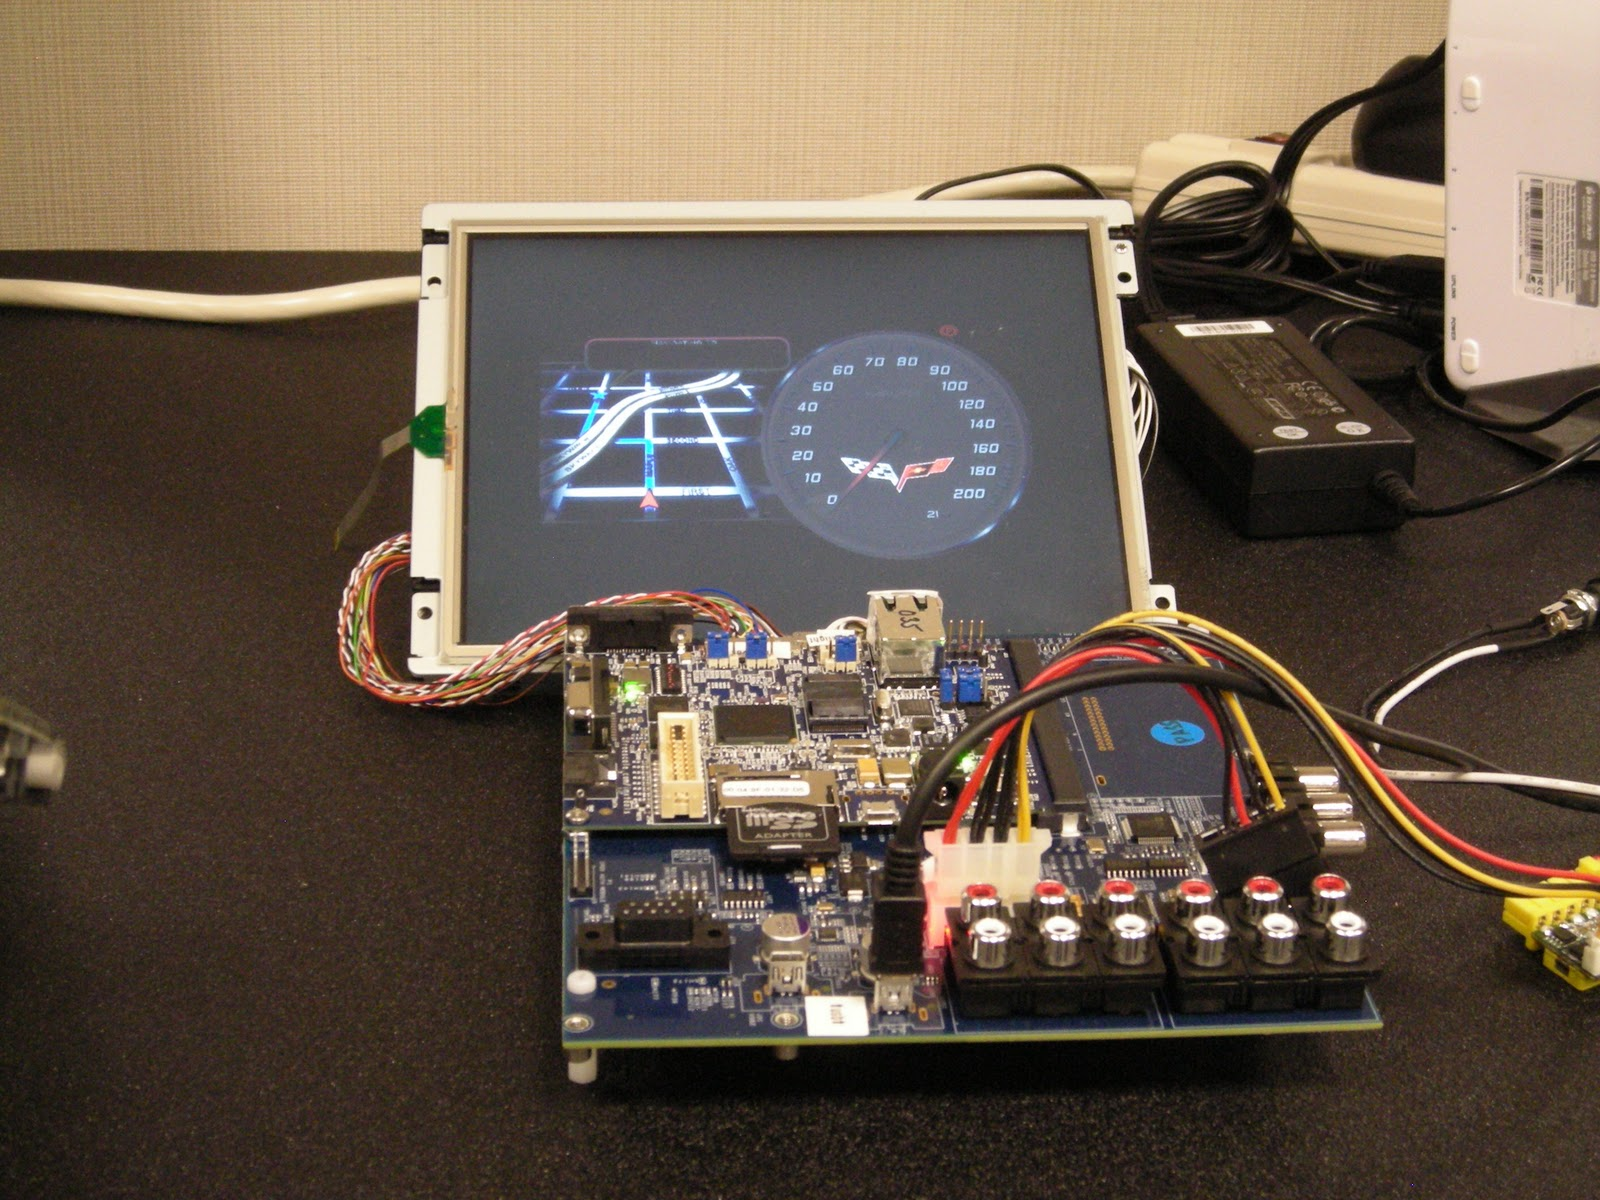
\includegraphics[width=6in]{sabre}
    \caption[The SABRE Platform]{The SABRE Platform}
    \label{ref:sabre}
\end{figure}

The standard method of communication between automotive controllers is CAN. This
protocol provides reliable communication that is suitable for high noise
environments such as an automobile. The SABRE platform provides one high speed
and one low speed CAN interface. These are implemented using the Freescale
FlexCAN peripheral, which is supported in the Linux kernel.

In the vehicle, the high speed CAN channel is used to communicate with the
battery management system and the vehicle's supervisory controller. By writing
software for the supervisory controller, messages can be sent to the center
stack over CAN. The low speed CAN channel is used to connect to the vehicle's
Heating, Ventilation, and Air Conditioning (HVAC) system. This allows the center
stack to control the stock HVAC system based on inputs to the touchscreen.

The touchscreen was also provided by Freescale Semiconductor. It is a 10.1 inch
tablet touchscreen, which communicates over a Low-voltage Differential Signaling
(LVDS) interface with the SABRE platform. The capacitive touch input is
processed by an eGalax controller, which is supported in the Linux kernel. The
screen is used in a portrait orientation so that it fits in the vehicle's
dashboard. This orientation maximizes available screen space while meeting the
space constraints of the stock vehicle dashboard.

The system is powered by the vehicle's 12 volt system. It was connected to the
auxiliary power port, often called the cigarette lighter port. This port is
only switched on when the vehicle's key is in the accessory or run states,
ensuring that the system cannot drain the vehicle's 12 volt battery when the car
is powered off. While connecting to this power source was convenient, it is not ideal
since the system must be turned off when the car is powered off. The system must
also start from a fully powered off state every time the car is started. In the
future, it may be necessary to change to an always on power source to allow the
system to control its own power state. This would allow for the system to use a
low power sleep or hibernate mode to enable a faster boot up time without taxing 
the car's 12 volt battery.

The platform also has support for Universal Serial Bus (USB) devices, and audio
output. These features have not yet been utilized, but will be useful for future
expansion. The team has considered adding additional hardware for connectivity.
A Wi-Fi interface could be connected through the USB port and allow for
communication with smartphones and computers near the vehicle. A cellular data
modem could also be connected via USB, and allow for access to the internet.
This additional hardware creates a wealth of new opportunities.

\section{Operating System}

The operating system for the system consists of three main components: the
bootloader, the kernel, and the root filesystem. These components are loaded
onto a memory card, which the system executes code from when it is powered on.

\subsection{Bootloader}

The bootloader is responsible for setting up the hardware immediately after it
is powered on. The system uses u-boot as it's bootloader. This bootloader was
chosen since Freescale provides a working image that supports the Linux kernel.

The bootloader allows for parameters to be passed to the Linux kernel. In order
to set the board up properly, the 'can0' argument must be passed to enable the
high speed CAN channel. Also, the correct video argument must be specified
depending on the device that is to be used. The bootloader settings can be
changed by connecting to the SABRE platform's serial port and sending commands to the
bootloader.

\subsection{Kernel}

The kernel is responsible for controlling the hardware during execution, and
providing a hardware abstraction layer for programs. The system uses the Linux
kernel. Linux was chosen since it provides support for all of the required
hardware. New versions of Linux provide support for the i.MX6Q which can be
enabled by compiling a custom kernel. Support for CAN and the Freescale FlexCAN
peripheral is also available in new kernels, along with support for the
eGalax touchscreen.

In order to support the SABRE hardware, a custom kernel had to be built. This
was done by using the latest kernel sources and selecting configuration options
for the i.MX6Q, eGalax touchscreen, and the FlexCAN peripheral.

QNX was evaluated as an alternative to Linux for this project. However, support
for CAN was not reliable. Since CAN is critical to the design of the system, it
was decided that QNX would not be a viable kernel for the project.

\subsection{Root Filesystem}

The kernel provides the basics for running a system, but the root filesystem
provides all of the other functionality. Freescale provides two options for root
filesystems: Ubuntu and Linux Target Image Builder (LTIB).

The Ubuntu root filesystem provided by Freescale is a full Ubuntu Desktop
system. It is the Oneiric Ocelot release, which is from October 2011, and will
not be supported in the near future. Since the desktop release is far too bloated
for the system, and support will soon be dropped, this was not an ideal
solution.

LTIB is provided by Freescale for users that wish to build their own root filesystem. It does
this by cross compiling software for the target. Unfortunately, much of the
software provided by LTIB is outdated. Also, LTIB does not provide a
packaging system to allow easy deployment of new software. For these reasons,
LTIB was not considered to be ideal.

Instead of using a provided root filesystem, the Ubuntu Core root filesystem was
used. This is a very minimal installation which includes a package manager. Due
to some challenges with deploying a Ubuntu Core root filesystem, a tool called
core-builder was created to build custom systems based on Ubuntu Core.

To make a system that can easily be deployed, the custom applications that are
to be run on the center stack are included with the root filesystem and deployed
as a single tarball. This ensures that all required files and dependencies are
provided. It also allows the system to easily be deployed to a new memory card
should one be lost or damaged.

\section{The core-builder Build System}

The Ubuntu Core root filesystem is distributed as a gzipped tarball containing
the minimal files needed to run the system. This system is very limited, and
intended to be expanded to meet the needs of the application. The core-builder
utility accomplishes the task of setting up a Ubuntu Core root filesystem on a
host computer such as a desktop or laptop. It then allows the user to install
packages and build a system suitable for the application. Finally, the user can
deploy this package to their target system.

To allow the filesystem to be manipulated on a host computer which uses a
different architecture than the target, QEMU user emulation is used. This type
of emulation allows binaries for a different architecture to be executed on the
host computer. For example, a x86 host operating system can be used to build the
root filesystem for the ARM target.

The tool is built using GNU Make. It builds a minimal system that has
support for networking and QEMU user emulation. Using a collection of
Makefiles, the tool executes the steps needed to set up the environment:

\begin{enumerate}
  \item Download the specified version of the tarball,
  \item Extract the tarball,
  \item Set up resolv.conf to allow for name server resolution,
  \item Move qemu-static-arm to the root filesystem to enable QEMU user
  emulation
\end{enumerate}

Once this is complete, the user can specify packages to install. The Debian
Advanced Package Tool (APT) will fetch and install the packages. The user can
also use other commands within the root filesystem on their host machine. This
allows for source to be compiled using a faster computer than the target, such
as a desktop. It also allows for the creation of new user accounts, so that
there are valid credentials on the system when it is loaded onto the target.

The core-builder tool has been released under the GNU Public License
\cite{ref:gpl}.
It will be provided to other teams in the EcoCAR 2 competition to assist in
setting up a root filesystem for the Freescale SABRE platform. Possible
improvements to include allowing more settings to be automatically configured,
providing support for automatically building packages from source, and providing
support for installing Debian packages that are not in the Ubuntu repository
from package files.

\section{Carserver}

In order to provide a bridge between applications running on the center stack
system and the vehicle's CAN bus, a custom daemon was created. This daemon uses
Socket CAN to communicate with the vehicle's CAN bus, and ZeroMQ to
communicate with other applications on the system. It consists of two separate
servers: Carpub and Carctl.

A number of inter-process communication tools were considered for the
implementation of Carserver. ZeroMQ was chosen for a number of reasons. First,
it is lightweight and can easily be run on the provided hardware. It also has
supporting libraries in a variety of languages. Finally, it is network based,
allowing the possibility of expanding to other devices over a traditional
Ethernet or WiFi network.

Carserver is written in C, which allows for access to CAN bus through standard
UNIX Sockets. In order to handle the multitasking required to run multiple
servers, POSIX Threading is used. The syslog daemon is used to log informative
and debug messages from the application. Using syslog allows the developer to
view debug messages over the hardware serial port, which is helpful during
debugging.

\begin{figure}
    \centering
    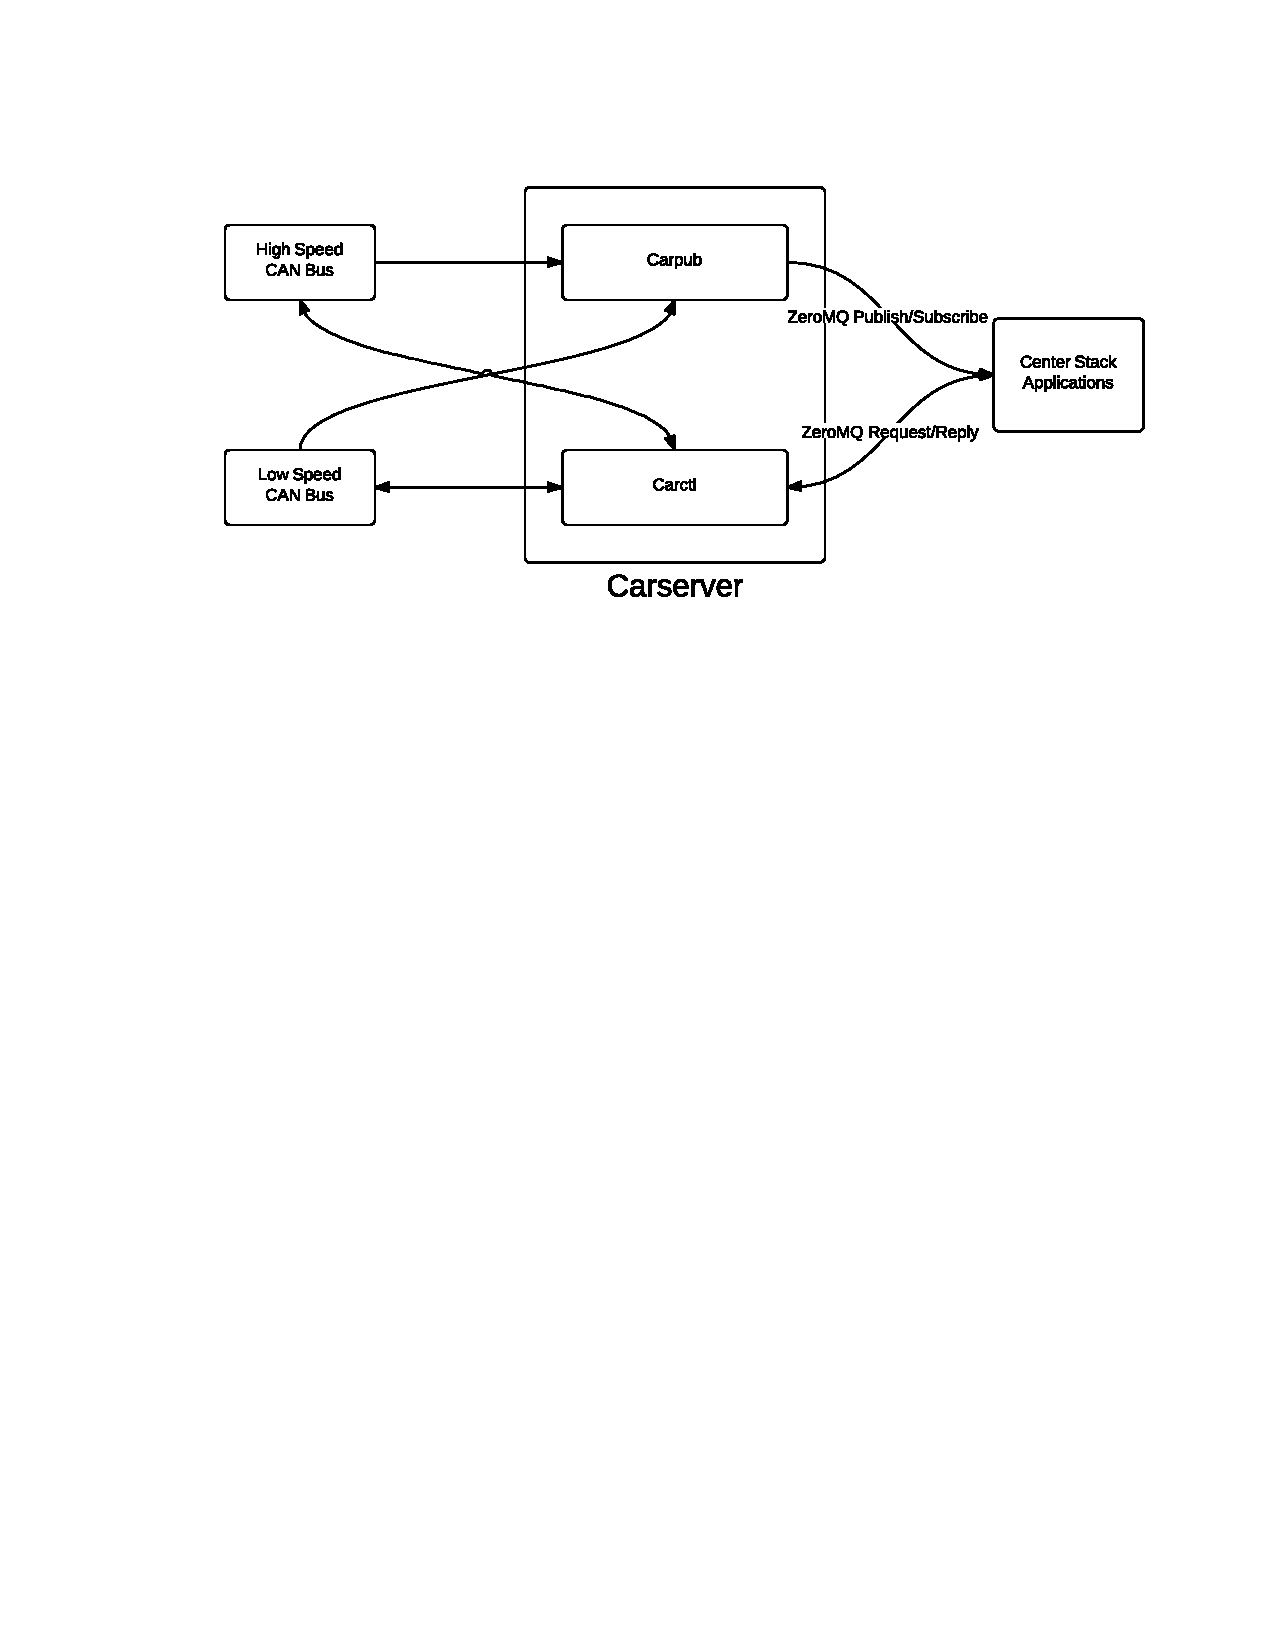
\includegraphics[height=7in]{carserver}
    \caption[The Carserver Architecture]{The Carserver Architecture}
    \label{ref:carserver}
\end{figure}

Using a server and client model for developing the system enabled the team to
parallelize the work. Once an interface was established, work on the server and
the GUI could be carried out at the same time. This allowed for more rapid
development of the center stack system. The architecture of Carserver is shown
in figure \ref{ref:carserver}.

There are many possible improvements to Carserver. Currently, filters for messages that
are to be received must be programmed into the application when it is compiled. This
could be replaced with a configuration file, which would allow for users to
change the settings without recompiling. Ideally, this configuration file would
be compatible with the standard CANdb file used by Vector CAN software.
Currently, Carserver uses no authentication, and instead depends on only trusted
devices being on the network. If untrusted devices are to be added to the
network, a new chain of trust must be established to prevent malicious activity.

\subsection{The Carpub Server}

In order to provide information to applications running on the center stack
system, Carpub publishes the most recent data seen on the CAN bus. It does this
by constantly listening to data on the bus and checking if it matches a rule. If
it does, it will perform the required conversion from the value on the bus to a
real unit by applying a specified offset and scale. The value will then be
stored in memory.

The purpose of Carpub is to be a publish only server. It does not allow the
client to send data. This enables the center stack to communicate with other
devices on the network, without introducing security risks. For example, the
center stack could publish data to a smartphone over a wireless network. While
this has not yet been implemented, it would be trivial to add the functionality
in year three of the competition.

For testing purposes, Carpub allows developers to put it into a fake data mode.
This mode does not connect to the CAN bus, but instead generates arbitrary data
that is sent to subscribing applications over the standard protocol. This mode
is useful for development and testing, since it allows application developers to
test their software without using the target hardware.

An example application of the Carpub server is to read the battery system's
state of charge and display it to the driver.

\subsection{The Carctl Server}

To control components in the vehicle, applications can use the Carctl server.
This server uses a request/response architecture. The client sends a request,
Carctl executes the matching routine, then sends a response. Each routine can
take arguments and return values to the requesting application. The current
implementation of Carctl is very minimal, but it can be expanded to control any
device on the high speed or low speed CAN bus in the future.

An example application of the Carctl server is to set the fan speed of the
vehicle's HVAC system. This is done by sending a specific message over the low
speed CAN bus. Access to Carctl can be limited to applications running locally
on the center stack, preventing malicious network access.

\section{The Graphical User Interface}

The system's GUI is implemented using Python and the pygame library.
These tools were chosen to allow for rapid development of a prototype GUI. The
GUI was primarily designed by Rickey Si Rui Wang. The GUI acts as a subscriber
to the Carpub server, and can send requests to the Carctl server.
Since the GUI and Carserver are completely separate applications, they could be
developed in parallel. By connecting to a Carserver sending fake data,
the GUI can be developed and tested on a desktop computer, then transfered to
the target hardware.

The GUI allows for the user to view information from the vehicle. It displays
the signals required by the EcoCAR 2 Non-Year Specific rules, and other messages
that are relevant to the operation of the vehicle. Since this is a prototype
vehicle, error codes can easily be displayed in the GUI. These codes assist with
debugging the vehicle's control logic during on-road testing. Safety critical
messages display as a full screen pop-up. This will alert the driver that
something has failed and safety precautions must be taken. For example, a low
high voltage isolation resistance, which indicates a ground fault of the
vehicle's high voltage bus, is displayed as a full screen pop-up. This is
critical since this type of fault greatly increases the chance of electric
shock and electrocution.

One challenge with developing the GUI was the GPU support on the Freescale
hardware. Unfortunately, hardware rendering is not currently supported. The team
plans to work with Freescale to resolve the issues, which will allow for more
complex GUIs to be built in the future. With hardware rendering support, a 3D
engine based on OpenGL could be utilized to create more impressive graphics.
Hardware video decoding would allow for seamless playback of compressed video
files. These types of features will be available once GPU support is
implemented, and could help to increase the consumer acceptability of the
vehicle. The current implementation of the GUI is shown in figure \ref{ref:gui}.

\begin{figure}
    \centering
    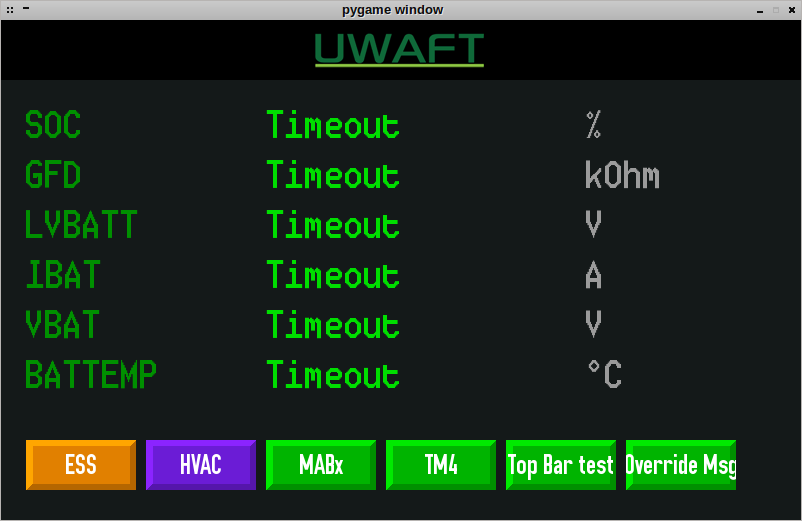
\includegraphics[width=6in]{gui}
    \caption[The Graphical User Interface]{The Graphical User Interface}
    \label{ref:gui}
\end{figure}

\section{Conclusions}

From the analysis in the report body, it is concluded that the University of
Waterloo Alternative Fuels Team now has a base system for their center stack
which can be improved upon. This system comprises of several components
including the hardware, operating system, low level software, and graphical user
interface. The modular design of the components will ease development in the
future.

The systems hardware has been implemented using the SABRE platform donated by
Freescale semiconductor, connected to the vehicle's auxiliary power, high speed
CAN bus, and low speed CAN bus. This allows for easy integration, and enables
the hardware to communicate with the various controllers in the vehicle.

The operating system uses the u-boot bootloader to initialize the hardware. It
then invokes the Linux kernel, which has been compiled for this specific
application. The kernel runs software from the root filesystem, which includes
the software needed for the center stack applications.

To ease with development of a root filesystem, core-builder was created. This
tool, based on GNU Make, allows the user to build Ubuntu Core based root
filesystem. This tool will be released to the other teams in the EcoCAR 2
competition, and will be released under an open source license to encourage
contribution.

The Carserver software handles dispatching data from the vehicle's CAN bus to
applications running on the center stack. It has two servers, one which
publishes data, and one that accepts requests. This system will also be given to
other EcoCAR 2 teams to aid with their center stack projects in the future.

The GUI for the system is based on Python and pygame, and is currently limited
by the lack of GPU support. This GUI is functional, but has many improvements
that could be made in the future. Due to the modular design of the system, the
GUI can be redesigned independently of the other system components.

\section{Recommendations}

The center stack system is currently in a prototype state, and several tools
have been developed to ease with future expansion. However, there a number of
next steps that could be taken to improve the system.

The current method of powering the system is less than ideal. It requires a full
shutdown every time the car is turned off. To solve this, an always on power
source could be used, and the system's hibernate mode could be initiated when
the car is powered off. This will prevent the system from draining the vehicle's
12 volt battery, but still allow for a fast start up time.

While Carctl provides basic support for controlling the vehicle, more
functionality could be added. This could include the ability to lock and unlock
doors, read GPS information from the vehicle's telematics controller, or adjust
vehicle settings.

To allow for more powerful GUI applications, the GPU support must be
implemented. The team should work with Freescale to rectify the issues with GPU
support.

There are many possibilities for future expansion by adding cellular network
access to the vehicle including telematics, maps, and social features. If these
are to be explored, the security of the system must be analysed.

Finally, to assist other teams in the EcoCAR 2 competition, the Carserver and
core-builder tools should be released under an open source license. To encourage
teams to contribute back to the projects, the GNU Public License \cite{ref:gpl} 
is suggested.

%%%%%%%%%%%%%%%%%%%%%%%%%%%%%%%%%%%%%%%%%%%%%%%%%%%%%%%%%%%%%%%%%%%%%
%% BACK MATTER
%%%%%%%%%%%%%%%%%%%%%%%%%%%%%%%%%%%%%%%%%%%%%%%%%%%%%%%%%%%%%%%%%%%%%
%% \backmatter will make the \section commands ignore their numbering,
\backmatter

% Here, we insert a References section, which will be formatted properly.
% The list of works you have referenced should be in FILENAME.bib,
% which will be workreport-sample.bib, if you use the command below.
%
% Note, you will need to process the document in a certain order.  First,
% run LaTeX.  The % first pass will allow LaTeX to build a list of 
% references, it may % emit warning messages such as:
%   LaTeX Warning: Reference `app:gnugpl' on page 4 undefined on input line 277.
%   LaTeX Warning: There were undefined references.
% This is normal.  Now you run BiBTeX in order to generate the proper
% layout for the references.  After this, you run LaTeX once more.
\bibliography{wkrpt}

%%%%%%%%%%%%%%%%%%%%%%%%%%%%%%%%%%%%%%%%%%%%%%%%%%%%%%%%%%%%%%%%%%%%%
%% APPENDICES
%%%%%%%%%%%%%%%%%%%%%%%%%%%%%%%%%%%%%%%%%%%%%%%%%%%%%%%%%%%%%%%%%%%%%
%% \appendix will reset \section numbers and turn them into letters.
%%
%% Don't forget to refer to all your appendices in the main report.
\appendix

\section{Glossary}\label{app:glossary}
\begin{description}
  \item[APT] Advanced Package Tool
  \item[CAN] Controller Area Network
  \item[CPU] Central Processing Unit
  \item[GPU] Graphics Processing Unit
  \item[GUI] Graphical User Interface
  \item[HVAC] Heating, Ventilation, and Air Conditioning
  \item[LVDS] Low-voltage Differential Signaling
  \item[POSIX] Portable Operating System Interface
  \item[SABRE] Smart Application Blueprint for Rapid Engineering
  \item[UWAFT] University of Waterloo Alternative Fuels Team
\end{description}

\end{document}
